\begin{name}
	{\tenchude}{\tendethi}{LỚP TOÁN THẦY PHÁT}{\thoigian}
\end{name}
\setcounter{ex}{0}
\Opensolutionfile{ans}[ans/ans-2-TT-24-LeThanhTong-NguyenKhuyen-HCM-23]
\begin{ex}%[Đề thi thử Tốt Nghiệp, Liên trường Lê Thánh Tông - Nguyễn Khuyến, HCM, 2023]%[12-EX-6-2023, Trần Quốc]%[2D2Y6-1]
Tập nghiệm của bất phương trình $2^x-5 \le 0$ là
\choice
{\True $S=\left(-\infty; \log_{2}{5}\right]$}
{$S=\left(0; \log_{2}{5}\right]$}
{$S=\left[0; \log_{2}{5}\right]$}
{$S=\left(0; \log_{5}{2}\right]$}
\loigiai{Ta có $2^x-5 \le 0 \Leftrightarrow 2^x\le 5 \Leftrightarrow x \le \log_{2}{5}$.\\
Suy ra tập nghiệm của bất phương trình đã cho là $S=\left(-\infty; \log_{2}{5}\right]$.}
\end{ex}

\begin{ex}%[Đề thi thử Tốt Nghiệp, Liên trường Lê Thánh Tông - Nguyễn Khuyến, HCM, 2023]%[12-EX-6-2023, Trần Quốc]%[2D1Y3-1]
Cho hàm số $y=f(x)$ liên tục trên đoạn $[-1; 3]$ và có bảng biến thiên như hình sau
\begin{center}

\begin{tikzpicture}
\tkzTabInit[nocadre=false,lgt=1.3,espcl=2.2,deltacl=0.6]
{$x$ /.6,$f'(x)$ /.6,$f(x)$/2}
{$-1$, $0$, $2$, $3$}
\tkzTabLine{,+,$0$,-,$0$,+,}
\tkzTabVar{-/$0$, +/$5$, -/$1$, +/$4$} 
\end{tikzpicture}
\end{center}
Giá trị lớn nhất của hàm số $y=f(x)$ trên đoạn $[-1; 3]$ bằng
\choice
{$3$}
{\True $5$}
{$0$}
{$4$}
\loigiai{Từ bảng biến thiên, ta có $f(x) \le 5$, $\forall x \in [-1; 3]$.\\
Suy ra $\max\limits_{[-1;3]}f(x)=f(0)=5$.}
\end{ex}

\begin{ex}%[Đề thi thử Tốt Nghiệp, Liên trường Lê Thánh Tông - Nguyễn Khuyến, HCM, 2023]%[12-EX-6-2023, Trần Quốc]%[2H3Y1-1]
Trong KG $Oxyz$, cho $\overrightarrow{OA}=2 \overrightarrow{i}+3 \overrightarrow{j}-\overrightarrow{k}$. Hình chiếu của $A$ lên mặt phẳng $(Oxz)$ là
\choice
{$M(2; 0; 3)$}
{$N(0;-1; 0)$}
{\True $P(2; 0;-1)$}
{$Q(0; 3; 0)$}
\loigiai{Ta có tọa độ điểm $A(2; 3; -1)$. \\
Do đó, hình chiếu của $A$ lên mặt phẳng $(Oxz)$ là $P(2;0;-1)$.}
\end{ex}

\begin{ex}%[Đề thi thử Tốt Nghiệp, Liên trường Lê Thánh Tông - Nguyễn Khuyến, HCM, 2023]%[12-EX-6-2023, Trần Quốc]%[2D3Y2-1]
Cho hàm số $f(x)=x^2-\dfrac{4}{x}$. Giá trị của $\int\limits_1^2 f'(x) \mathrm{\, d} x$ bằng
\choice
{$3$}
{\True $5$}
{$\dfrac{7}{3}$}
{$\dfrac{7}{3}-\ln 2$}
\loigiai{Ta có $\int\limits_1^2 f'(x) \mathrm{\, d} x=f(x)\Big|_{1}^{2}=f(2)-f(1)=\left(2^2-\dfrac{4}{2}\right)-\left(1^2-\dfrac{4}{1}\right)=5$.}
\end{ex}

\begin{ex}%[Đề thi thử Tốt Nghiệp, Liên trường Lê Thánh Tông - Nguyễn Khuyến, HCM, 2023]%[12-EX-6-2023, Trần Quốc]%[2D1Y5-1]
\immini{Hàm số nào sau đây có đồ thị như hình vẽ ở bên?
\choice
{$y=\dfrac{x+2}{x}$}
{$y=\dfrac{2 x+1}{x-2}$}
{\True $y=\dfrac{x+2}{x-2}$}
{$y=\dfrac{2 x+4}{2 x-2}$}}
{
\begin{tikzpicture}[font=\footnotesize,line join=round, line cap=round, >=stealth,scale=0.4] 
\def \xmin{-4}\def \xmax{8}\def \ymin{-3}\def \ymax{5}
\draw[->] (\xmin,0)--(\xmax,0) node[shift=(-90:0.25)] {$x$};
\draw[->] (0,\ymin)--(0,\ymax) node[shift=(0:0.25)] {$y$};
\fill (0,0) circle(2pt) node[shift=(-45:0.25)]{$O$}
		(-2,0) circle(2pt) node[shift=(-90:0.2)]{$-2$}
		(2,0) circle(2pt) node[shift=(-45:0.25)]{$2$}
		(0,-1) circle(2pt) node[shift=(-150:0.25)]{$-1$}
		(0,1) circle(2pt) node[shift=(135:0.2)]{$1$};
\draw[dashed] (\xmin,1)--(\xmax,1) (2,\ymin)--(2,\ymax);
\begin{scope}
\clip (\xmin,\ymin) rectangle (\xmax,\ymax);
\draw[smooth,samples=100,domain=\xmin:1.9] plot(\x,{(\x+2)/(\x-2)}); 
\draw[smooth,samples=100,domain=2.1:\xmax] plot(\x,{(\x+2)/(\x-2)}); 
\end{scope}
\end{tikzpicture}}
\loigiai{Từ đồ thị, ta có nhận xét:
\begin{itemize}
\item Đồ thị hàm số có đường tiệm cận đứng $x=2$ và đường tiệm cận ngang $y=1$;
\item Đồ thị cắt trục hoành tại điểm có hoành độ $x=-2$ và cắt trục tung tại điểm có tung độ $y=-1$.
\end{itemize}
Do đó, phương án đúng là hàm số $y=\dfrac{x+2}{x-2}$.
}
\end{ex}

\begin{ex}%[Đề thi thử Tốt Nghiệp, Liên trường Lê Thánh Tông - Nguyễn Khuyến, HCM, 2023]%[12-EX-6-2023, Trần Quốc]%[2H3Y3-1]
Trong KG $Oxyz$, cho hai mặt phẳng $(P) \colon x-2 y+z-3=0$ và $(Q) \colon x+y-1=0$. Giao tuyến của $(P)$ và $(Q)$ có một véc-tơ chỉ phương là
\choice
{$\overrightarrow{u}=(1; 0;-1)$}
{\True $\overrightarrow{u}=(1;-1;-3)$}
{$\overrightarrow{u}=(3; 0;-1)$}
{$\overrightarrow{u}=(1; 1;-3)$}
\loigiai{
\begin{itemize}
\item Mặt phẳng $(P)$ có một véc-tơ pháp tuyến là $\overrightarrow{n}_{P}=(1;-2;1)$.
\item Mặt phẳng $(Q)$ có một véc-tơ pháp tuyến là $\overrightarrow{n}_{Q}=(1;1;0)$.
\end{itemize}
Do đó, giao tuyến của $(P)$ và $(Q)$ có một véc-tơ chỉ phương là $\overrightarrow{u}=\left[\overrightarrow{n}_{Q}; \overrightarrow{n}_{P}\right]=(1;-1;-3)$.
}
\end{ex}

\begin{ex}%[Đề thi thử Tốt Nghiệp, Liên trường Lê Thánh Tông - Nguyễn Khuyến, HCM, 2023]%[12-EX-6-2023, Trần Quốc]%[2D1Y2-2]
Cho hàm số $y=f(x)$ có bảng biến thiên như hình 
\begin{center}

\begin{tikzpicture}
\tkzTabInit[nocadre=false,lgt=1.3,espcl=2.2,deltacl=0.6] 
{$x$ /.6,$f'(x)$ /.6,$f(x)$/2}
{$-\infty$, $-1$, $1$,$+\infty$}
\tkzTabLine{,+,$0$,-,$0$,+,}
\tkzTabVar{-/$-\infty$, +/$2$, -/$-2$, +/$+\infty$}
\end{tikzpicture}
\end{center}
Điểm cực đại của hàm số $y=f(x)$ là
\choice
{$x=2$}
{$y=2$}
{$y=-1$}
{\True $x=-1$}
\loigiai{Dựa vào bảng biến thiên, suy ra hàm số đạt cực đại tại $x=-1$.}
\end{ex}

\begin{ex}%[Đề thi thử Tốt Nghiệp, Liên trường Lê Thánh Tông - Nguyễn Khuyến, HCM, 2023]%[12-EX-6-2023, Trần Quốc]%[2H2Y1-2]
Một hình nón có chiều cao là $h$ và bán kính của đường tròn đáy bằng $R$. Diện tích xung quanh của hình nón đó bằng
\choice
{$2 \pi R h$}
{$\pi R h$}
{$2 \pi R \sqrt{h^2+R^2}$}
{\True $\pi R \sqrt{h^2+R^2}$}
\loigiai{
Hình nón có đường sinh $\ell=\sqrt{h^2+r^2}$.\\
Suy ra diện tích xung quanh của hình nón là $S_{\text{xq}}=\pi R \ell =\pi R \sqrt{h^2+r^2}$.}
\end{ex}

\begin{ex}%[Đề thi thử Tốt Nghiệp, Liên trường Lê Thánh Tông - Nguyễn Khuyến, HCM, 2023]%[12-EX-6-2023, Trần Quốc]%[2H3Y2-2]
Trong KG $Oxyz$, một véc-tơ pháp tuyến mặt phẳng $(Oxz)$ có tọa độ là
\choice
{$(0; 1; 1)$}
{$(1; 0; 1)$}
{\True $(0; 1; 0)$}
{$(1; 0; 0)$}
\loigiai{Một véc-tơ pháp tuyến của mặt phẳng $(Oxz)$ là $\overrightarrow{j}=(0; 1; 0)$.}
\end{ex}

\begin{ex}%[Đề thi thử Tốt Nghiệp, Liên trường Lê Thánh Tông - Nguyễn Khuyến, HCM, 2023]%[12-EX-6-2023, Trần Quốc]%[2H1Y3-2]
Thể tích khối lăng trụ có diện tích đáy $B=20 \text{~cm}^2$ và chiều cao $h=3 \text{~cm}$ là
\choice
{$V=23 \text{~cm}^3$}
{$V=20 \text{~cm}^3$}
{\True $V=60 \text{~cm}^3$}
{$V=45 \text{~cm}^3$}
\loigiai{
Thể tích khối lăng trụ đã cho là $V=Bh=20\cdot 3=60 \text{~cm}^3$.
}
\end{ex}

\begin{ex}%[Đề thi thử Tốt Nghiệp, Liên trường Lê Thánh Tông - Nguyễn Khuyến, HCM, 2023]%[12-EX-6-2023, Trần Quốc]%[2D1Y2-2]
Cho hàm số $y=f(x)$ liên tục trên $\mathbb{R}$ và có bảng xét dấu đạo hàm như hình sau
\begin{center}

\begin{tikzpicture}
\tkzTabInit[nocadre=false,lgt=1.3,espcl=2.2,deltacl=0.6]
{$x$ /.6,$f'(x)$ /.6}
{$-\infty$, $-1$, $0$, $1$, $2$,$+\infty$}
\tkzTabLine{,+,$0$,-,$0$,+,d,-,$0$,+,}
\end{tikzpicture}
\end{center}
Hàm số đã cho có bao nhiêu điểm cực đại?
\choice
{\True $2$}
{$3$}
{$4$}
{$1$}
\loigiai{
Ta có bảng biến thiên của hàm số $y=f(x)$
\begin{center}

\begin{tikzpicture}
\tkzTabInit[nocadre=false,lgt=1.3,espcl=2.2,deltacl=0.6]
{$x$ /.6,$f'(x)$ /.6,$f(x)$/2}
{$-\infty$, $-1$, $0$, $1$, $2$,$+\infty$}
\tkzTabLine{,+,$0$,-,$0$,+,d,-,$0$,+,}
\tkzTabVar{-/,+/, -/, +/, -/, +/} 
\end{tikzpicture}
\end{center}
Vì hàm số $y=f(x)$ liên tục trên $\mathbb{R}$ nên hàm số có hai điểm cực đại là $x=-1$ và $x=1$.
}
\end{ex}

\begin{ex}%[Đề thi thử Tốt Nghiệp, Liên trường Lê Thánh Tông - Nguyễn Khuyến, HCM, 2023]%[12-EX-6-2023, Trần Quốc]%[2D2Y4-3]
Hàm số nào sau đây luôn đồng biến trên $\mathbb{R}$?
\choice
{$f(x)=x^2+3$}
{$f(x)=x^4+x^2$}
{\True $f(x)=\left(\dfrac{\pi}{3}\right)^x$}
{$f(x)=(\log 5)^x$}
\loigiai{Xét hàm số $f(x)=\left(\dfrac{\pi}{3}\right)^x$ trên $\mathbb{R}$.\\
Ta có $f'(x)=\left(\dfrac{\pi}{3}\right)^x \ln \dfrac{\pi}{3}>0$, $\forall x \in \mathbb{R}$.\\
Do đó, hàm số $f(x)=\left(\dfrac{\pi}{3}\right)^x$ luôn đồng biến trên $\mathbb{R}$.} 
\end{ex}

\begin{ex}%[Đề thi thử Tốt Nghiệp, Liên trường Lê Thánh Tông - Nguyễn Khuyến, HCM, 2023]%[12-EX-6-2023, Trần Quốc]%[1D3Y3-3]
Các số $5$, $a$, $9$, $b$ theo thứ tự lập thành một cấp số cộng. Khi đó
\choice
{$ab=60$}
{$ab=96$}
{$ab=72$}
{\True $ab=77$}
\loigiai{Cấp số cộng đã cho có $\heva{&u_1=5 \\&u_3=9.}$ \\
Do đó $2d=u_3-u_1=9-5=4 \Rightarrow d=2$.\\
Suy ra $a=u_2=u_1+d=7$ và $b=u_4=u_3+d=11$.\\
Vậy $ab=77$.}
\end{ex}

\begin{ex}%[Đề thi thử Tốt Nghiệp, Liên trường Lê Thánh Tông - Nguyễn Khuyến, HCM, 2023]%[12-EX-6-2023, Trần Quốc]%[2D2Y4-3]
Tiệm cận ngang của đồ thị của hàm số $y=5^x$ có phương trình
\choice
{$x=0$}
{$y=5$}
{\True $y=0$}
{$x=5$}
\loigiai{Vì $\lim\limits_{x \to +\infty}y=\lim\limits_{x \to +\infty}5^x=+\infty$ và $\lim\limits_{x \to -\infty}y=\lim\limits_{x \to -\infty}5^x=0$ nên đồ thị của hàm số $y=5^x$ có đúng một đường tiệm cận ngang là $y=0$.}
\end{ex}

\begin{ex}%[Đề thi thử Tốt Nghiệp, Liên trường Lê Thánh Tông - Nguyễn Khuyến, HCM, 2023]%[12-EX-6-2023, Trần Quốc]%[2H3Y1-3]
Trong KG $Oxyz$, mặt cầu $(S)\colon x^2+y^2+z^2-4x+6y-3=0$ có diện tích bằng
\choice
{$120 \pi$}
{$40 \pi$}
{$32 \pi$}
{\True $64 \pi$}
\loigiai{Mặt cầu $(S)$ có tâm $I(2;-3;0)$ và bán kính $R=\sqrt{2^2+(-3)^2+0^2-(-3)}=4$.\\
Do đó, mặt cầu $(S)$ có diện tích là $S=4\pi R^2=64\pi$.}
\end{ex}

\begin{ex}%[Đề thi thử Tốt Nghiệp, Liên trường Lê Thánh Tông - Nguyễn Khuyến, HCM, 2023]%[12-EX-6-2023, Trần Quốc]%[2H3Y2-3]
Trong KG $Oxyz$, mặt phẳng đi qua ba điểm $A(1; 0; 0)$, $B(0; 2; 0)$, $C(0; 0;-4)$ có phương trình là
\choice
{$\dfrac{x}{1}+\dfrac{y}{2}-\dfrac{z}{4}=0$}
{$\dfrac{x}{1}+\dfrac{y}{2}+\dfrac{z}{4}=1$}
{\True $\dfrac{x}{1}+\dfrac{y}{2}-\dfrac{z}{4}=1$}
{$-\dfrac{x}{1}+\dfrac{y}{2}+\dfrac{z}{4}=1$}
\loigiai{Mặt phẳng $(ABC)$ có phương trình đoạn chắn là $\dfrac{x}{1}+\dfrac{y}{2}-\dfrac{z}{4}=1$.}
\end{ex}

\begin{ex}%[Đề thi thử Tốt Nghiệp, Liên trường Lê Thánh Tông - Nguyễn Khuyến, HCM, 2023]%[12-EX-6-2023, Trần Quốc]%[2D2Y5-3]
Nếu đặt $t=\log x$ thì bất phương trình $\log^2x^3-10\log\sqrt{x}+1\ge 0$ trở thành
\choice
{$3t^2+1 \ge 0$}
{$3t^2-5t+1 \ge 0$}
{\True $9t^2-5t+1 \ge 0$}
{$9t^2-20t+1 \ge 0$}
\loigiai{
Điều kiện $x>0$.\\
Ta có
$$\log^2x^3-10\log \sqrt{x}+1 \ge 0 \Leftrightarrow 9 \log ^2x-5\log x+1 \ge 0.$$
Đặt $t=\log x$, phương trình trở thành $9t^2-5t+1 \ge 0$.}
\end{ex}

\begin{ex}%[Đề thi thử Tốt Nghiệp, Liên trường Lê Thánh Tông - Nguyễn Khuyến, HCM, 2023]%[12-EX-6-2023, Trần Quốc]%[2D1Y5-4]
Đồ thị của hàm số $y=\left(x^2-4\right)(x+2)^2$ cắt trục hoành tại bao nhiêu điểm phân biệt?
\choice
{\True $2$}
{$3$}
{$4$}
{$1$}
\loigiai{Xét phương trình hoành độ giao điểm
$$ \left(x^2-4\right)(x+2)^2=0\Leftrightarrow \hoac{&x^2-4=0 \\&x+2=0} \Leftrightarrow \hoac{&x=2 \\&x=-2.}$$
Vậy đồ thị hàm số đã cho cắt trục hoành tại hai điểm phân biệt.
}
\end{ex}

\begin{ex}%[Đề thi thử Tốt Nghiệp, Liên trường Lê Thánh Tông - Nguyễn Khuyến, HCM, 2023]%[12-EX-6-2023, Trần Quốc]%[2D1B1-1]
Tìm khoảng nghịch biến của hàm số $y=f(x)$, biết $f'(x)=(x-3)(x+2)(x+5)^2$, $\forall x \in \mathbb{R}$.
\choice
{$(-\infty;-5)$}
{\True $(-2; 3)$}
{$(-5;-2)$}
{$(3;+\infty)$}
\loigiai{Ta có $f'(x)=0 \Leftrightarrow (x-3)(x+2)(x+5)^2=0 \Leftrightarrow \hoac{&x=3 \\&x=-2 \\&x=-5 \quad \text{(nghiệm kép)}.}$\\
Bảng biến thiên của hàm số $y=f(x)$
\begin{center}

\begin{tikzpicture}
\tkzTabInit[nocadre=false,lgt=1.3,espcl=2.2,deltacl=0.6] 
{$x$ /.6,$f'(x)$ /.6,$f(x)$/2}
{$-\infty$, $-5$, $-2$, $3$, $+\infty$}
\tkzTabLine{,+,$0$,+,$0$,-,$0$,+,}
\tkzTabVar{-/$-\infty$, R, +/,  -/, +/$+\infty$} 
\end{tikzpicture}
\end{center}
Dựa vào bảng biến thiên, ta có hàm số nghịch biến trên khoảng $(-2;3)$.
}
\end{ex}

\begin{ex}%[Đề thi thử Tốt Nghiệp, Liên trường Lê Thánh Tông - Nguyễn Khuyến, HCM, 2023]%[12-EX-6-2023, Trần Quốc]%[2D2B2-1]
Hàm số nào sau đây có tập xác định là $\mathbb{R}$?
\choice
{$y=x^{-2}$}
{\True $y=\sqrt[5]{x^3}$}
{$y=x^{2 \pi}$}
{$y=x^{\tfrac{1}{3}}$}
\loigiai{Hàm số có tập xác định $\mathscr{D}=\mathbb{R}$ là $y=\sqrt[5]{x^3}$.}
\end{ex}

\begin{ex}%[Đề thi thử Tốt Nghiệp, Liên trường Lê Thánh Tông - Nguyễn Khuyến, HCM, 2023]%[12-EX-6-2023, Trần Quốc]%[2D3B1-1]
Khẳng định nào sau đây là đúng?
\choice
{$\int \cos x \mathrm{\, d} x=-\sin x+C$}
{$\int x^5 \mathrm{\, d} x=\dfrac{1}{5} x^6+C$}
{$\int \mathrm{e}^x \mathrm{\, d} x=\dfrac{\mathrm{e}^{x+1}}{x+1}+C$, $\forall x \neq-1$}
{\True $\int \dfrac{1}{x} \mathrm{\, d} x=\ln |2023 x|+C$}
\loigiai{Vì $\ln |2023x| +C=\ln |x|+\left(\ln 2023+C\right)$, $\forall x \ne 0$ nên ta có khẳng định đúng là $\int \dfrac{1}{x} \mathrm{\, d} x=\ln |2023 x|+C$.}
\end{ex}

\begin{ex}%[Đề thi thử Tốt Nghiệp, Liên trường Lê Thánh Tông - Nguyễn Khuyến, HCM, 2023]%[12-EX-6-2023, Trần Quốc]%[2D3B3-1]
Gọi $(H)$ là hình phẳng giới hạn bởi các đường $y=0$; $x=1$; $x=5$; $y=\mathrm{e}^x$. Thể tích $V$ của khối tròn xoay tạo thành khi quay $(H)$ quanh trục $Ox$ là
\choice
{$V=\pi \int\limits_1^5 \mathrm{e}^{x+1} \mathrm{\, d} x$}
{$V=\pi \int\limits_1^5 \mathrm{e}^{x^2} \mathrm{\, d} x$}
{\True $V=\pi \int\limits_1^5 \mathrm{e}^{2 x} \mathrm{\, d} x$}
{$V=\pi^2 \int\limits_1^5 \mathrm{e}^x \mathrm{\, d} x$}
\loigiai{Thể tích $V$ của khối tròn xoay tạo thành khi quay $(H)$ quanh trục $Ox$ là
$V=\pi \int\limits_1^5 \mathrm{e}^{2 x} \mathrm{\, d} x$.}
\end{ex}

\begin{ex}%[Đề thi thử Tốt Nghiệp, Liên trường Lê Thánh Tông - Nguyễn Khuyến, HCM, 2023]%[12-EX-6-2023, Trần Quốc]%[2D3B3-1]
\immini{Cho hàm số $y=f(x)$ có đồ thị như hình vẽ. Diện tích của hình phẳng gạch chéo trong hình được tính bởi công thức nào?
\choice
{$S=\int\limits_0^{-3} f(x) \mathrm{\, d} x-\int\limits_0^4 f(x) \mathrm{\, d} x$}
{$S=\int\limits_{-3}^0 f(x) \mathrm{\, d} x+\int\limits_0^4 f(x) \mathrm{\, d} x$}
{\True $S=\int\limits_{-3}^0 f(x) \mathrm{\, d} x-\int\limits_0^4 f(x) \mathrm{\, d} x$}
{$S=\left|\int\limits_{-3}^4 f(x) \mathrm{\, d} x\right|$}}
{
\begin{tikzpicture}[font=\footnotesize,line join=round, line cap=round, >=stealth,scale=0.7] 
\def \xmin{-4}\def \xmax{5}\def \ymin{-2.5}\def \ymax{2}
\draw[->] (\xmin,0)--(\xmax,0) node[shift=(-90:0.25)] {$x$};
\draw[->] (0,\ymin)--(0,\ymax) node[shift=(0:0.25)] {$y$};
\fill (0,0) circle(1pt) node[shift=(-135:0.25)]{$O$}
		(-3,0) circle(1pt) node[shift=(135:0.25)]{$-3$}
		(4,0) circle(1pt) node[shift=(-45:0.25)]{$4$}; 
\begin{scope}
\clip (\xmin,\ymin) rectangle (\xmax,\ymax); 
\draw[smooth,samples=100,domain=\xmin:\xmax] plot(\x,{(\x)*(\x+3)*(\x-4)/10}); 
\fill[pattern = north west lines,opacity=.5] plot[domain=0:4](\x,{(\x)*(\x+3)*(\x-4)/10})--(0,0)--(-3,0)--plot[domain=-3:0](\x,{(\x)*(\x+3)*(\x-4)/10});
\end{scope} 
\end{tikzpicture}}
\loigiai{Diện tích hình phẳng gạch chéo được tính bởi công thức
$$\int\limits_{-3}^{4}\left|f(x)\right| \mathrm{\, d} x =\int\limits_{-3}^0 f(x) \mathrm{\, d} x-\int\limits_0^4 f(x) \mathrm{\, d} x.$$}
\end{ex}

\begin{ex}%[Đề thi thử Tốt Nghiệp, Liên trường Lê Thánh Tông - Nguyễn Khuyến, HCM, 2023]%[12-EX-6-2023, Trần Quốc]%[2D1B4-1]
Số đường tiệm cận đứng của đồ thị hàm số $y=\dfrac{\sqrt{x}}{x\left(x^2-2\right)}$ là
\choice
{\True $2$}
{$1$}
{$3$}
{$0$}
\loigiai{Tập xác định $\mathscr{D}=(0;+\infty) \setminus \left\{\sqrt{2}\right\}$.\\
Ta có
\begin{itemize}
\item $\lim\limits_{x \to 0^+}y=\lim\limits_{x \to 0^+} \dfrac{\sqrt{x}}{x\left(x^2-2\right)}=\lim\limits_{x \to 0^+} \dfrac{1}{\sqrt{x}\left(x^2-2\right)}=-\infty$;
\item $\lim\limits_{x \to \sqrt{2}^+}y=\lim\limits_{x \to \sqrt{2}^+} \dfrac{\sqrt{x}}{x\left(x^2-2\right)}=\lim\limits_{x \to \sqrt{2}^+} \dfrac{1}{\sqrt{x}\left(x^2-2\right)}=+\infty$;
\item $\lim\limits_{x \to \sqrt{2}^-}y=\lim\limits_{x \to \sqrt{2}^-} \dfrac{\sqrt{x}}{x\left(x^2-2\right)}=\lim\limits_{x \to \sqrt{2}^-} \dfrac{1}{\sqrt{x}\left(x^2-2\right)}=-\infty$.
\end{itemize}
Suy ra đồ thị hàm số đã cho có $2$ đường tiệm cận đứng là $x=0$ và $x=\sqrt{2}$.}
\end{ex}

\begin{ex}%[Đề thi thử Tốt Nghiệp, Liên trường Lê Thánh Tông - Nguyễn Khuyến, HCM, 2023]%[12-EX-6-2023, Trần Quốc]%[2D3B2-1]
Cho hàm số $y=f(x)$ có đạo hàm trên $(0;+\infty)$. Biết $g(x)=3x^2$ là một nguyên hàm của $x^2 f'(x)$ trên $(0;+\infty)$ và $f(1)=2$. Tính giá trị $f(\mathrm{e})$.
\choice
{\True $f(\mathrm{e})=8$}
{$f(\mathrm{e})=6 \mathrm{e}-2$}
{$f(\mathrm{e})=4$}
{$f(\mathrm{e})=3 \mathrm{e}+2$}
\loigiai{Vì $g(x)=3x^2$ là một nguyên hàm của $x^2 f'(x)$ nên ta có
$$ x^2 f'(x)=g'(x)=\left(3x^2\right)'=6x \Rightarrow f'(x)=\dfrac{6}{x}, \forall x \in (0; +\infty). $$
Do đó $f(\mathrm{e})-f(1)=\int\limits_{1}^{\mathrm{e}} f'(x) \mathrm{\, d} x=\int\limits_{1}^{\mathrm{e}}\dfrac{6}{x} \mathrm{\, d} x =6\ln x\Big|_{1}^{\mathrm{e}}=6$.\\
Vậy $f(\mathrm{e})=6+f(1)=8$.
}
\end{ex}

\begin{ex}%[Đề thi thử Tốt Nghiệp, Liên trường Lê Thánh Tông - Nguyễn Khuyến, HCM, 2023]%[12-EX-6-2023, Trần Quốc]%[2D2B5-2]
Số nghiệm thực của phương trình $1+\ln (x+3)-\ln (x-1)^2=0$ là
\choice
{\True $2$}
{$1$}
{$0$}
{$3$}
\loigiai{Điều kiện $\heva{&x+3 >0 \\& (x-1)^2>0} \Leftrightarrow \heva{&x>-3 \\&x \ne 1.}$\\
Khi đó, phương trình đã cho tương đương
\[\ln (x-1)^2-\ln (x+3)=1 \Leftrightarrow \ln \dfrac{\left(x-1\right)^2}{x+3}=1 \Leftrightarrow \dfrac{\left(x-1\right)^2}{x+3}=\mathrm{e}.\]
Xét hàm số $f(x)=\dfrac{(x-1)^2}{x+3}$ trên $(-3;+\infty)$.\\
Ta có $f'(x)=\dfrac{x^2+6x-7}{(x+3)^2}$.\\
Phương trình $f'(x)=0 \Leftrightarrow x^2+6x-7=0 \Leftrightarrow \hoac{&x=1 & \\&x=-7 &\text{(loại).}}$\\
Bảng biến thiên hàm số $y=f(x)$ trên khoảng $(-3;+\infty)$
\begin{center}

\begin{tikzpicture}
\tkzTabInit[nocadre=false,lgt=1.3,espcl=2.2,deltacl=0.6] 
{$x$ /.6,$f'(x)$ /.6,$f(x)$/2}
{$-3$, $1$,$+\infty$}
\tkzTabLine{,-,0,+,}
\tkzTabVar{+/$+\infty$, -/$0$, +/$+\infty$} 
\end{tikzpicture}
\end{center}
Từ bảng biến thiên hàm số $y=f(x)$ trên khoảng $(-3;+\infty)$, suy ra phương trình $f(x)=\mathrm{e}$ có đúng $2$ nghiệm thực thuộc khoảng $(-3;+\infty) \setminus \{1\}$.\\
Vậy phương trình đã cho có đúng $2$ nghiệm thực phân biệt.
}
\end{ex}

\begin{ex}%[Đề thi thử Tốt Nghiệp, Liên trường Lê Thánh Tông - Nguyễn Khuyến, HCM, 2023]%[12-EX-6-2023, Trần Quốc]%[2H3B3-2]
Trong KG $Oxyz$, đường thẳng $\Delta$ đi qua điểm $M(1; 0;-2)$ và vuông góc với mặt phẳng $(Q) \colon 4x+y-3z+2023=0$ có PTTS là
\def\dotEX{}
\choice
{$\heva{&x=1+4t \\ &y=-t \\ &z=2-3t.}$}
{\True $\heva{&x=-3+4t \\ &y=-1+t \\ &z=1-3t.}$}
{$\heva{&x=1-4t \\ &y=t \\ &z=-2-3t.}$}
{$\heva{&x=1-4t \\ &y=0 \\ &z=-2+3t.}$}
\loigiai{Vì đường thẳng $\Delta$ vuông góc với mặt phẳng $(Q)$ nên có một véc-tơ chỉ phương là $\overrightarrow{u}_{\Delta}=\overrightarrow{n}_{P}=(4;1;-3)$.\\
Mặt khác, $\Delta$ qua $M(1;0;-2)$ nên có PTTS là $\heva{&x=1+4t \\&y=t \\&z=-2-3t.}$\\
Với $t=-1$, đường thẳng $\Delta$ cũng qua điểm $N(-3;-1;1)$.\\
Do đó, $\Delta$ cũng có PTTS là $\heva{&x=-3+4t \\ &y=-1+t \\ &z=1-3t.}$
}
\end{ex}

\begin{ex}%[Đề thi thử Tốt Nghiệp, Liên trường Lê Thánh Tông - Nguyễn Khuyến, HCM, 2023]%[12-EX-6-2023, Trần Quốc]%[2D1B1-2]
\immini{Cho hàm số $y=f(x)$ xác định và liên tục trên $\mathbb{R}$ có đồ thị hàm số $y=f'(x)$ như hình vẽ bên. Hàm số $y=f(x+2)$ nghịch biến trên khoảng nào sau đây?
\choice
{$(-\infty;-4)$}
{$(-2; 0)$}
{\True $(-4;-2)$}
{$(-2;+\infty)$}}
{
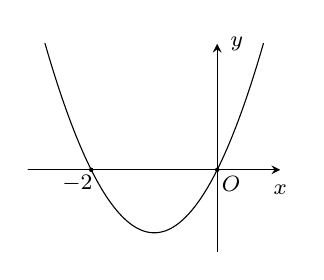
\begin{tikzpicture}[font=\footnotesize,line join=round, line cap=round, >=stealth,scale=0.8] 
\def \xmin{-3}\def \xmax{1}\def \ymin{-1.3}\def \ymax{2}
\draw[->] (\xmin,0)--(\xmax,0) node[shift=(-90:0.25)] {$x$};
\draw[->] (0,\ymin)--(0,\ymax) node[shift=(0:0.25)] {$y$};
\fill (0,0) circle(1pt) node[shift=(-45:0.25)]{$O$}
		(-2,0) circle(1pt) node[shift=(-135:0.25)]{$-2$};
\begin{scope}
\clip (\xmin,\ymin) rectangle (\xmax,\ymax); 
\draw[smooth,samples=100,domain=\xmin:\xmax] plot(\x,{(\x)*(\x+2)}); 
\end{scope}  
\end{tikzpicture}}
\loigiai{
Xét hàm số $g(x)=f(x+2)$ trên $\mathbb{R}$.\\
Ta có $g'(x)=f'(x+2)$.\\
Khi đó $g'(x)<0 \Leftrightarrow f'(x+2)<0 \Leftrightarrow -2<x+2<0 \Leftrightarrow -4<x<-2$.\\
Suy ra hàm số $y=f(x+2)$ nghịch biến trên khoảng $(-4;2)$.
}
\end{ex}

\begin{ex}%[Đề thi thử Tốt Nghiệp, Liên trường Lê Thánh Tông - Nguyễn Khuyến, HCM, 2023]%[12-EX-6-2023, Trần Quốc]%[2D3B2-2]
Thực hiện phép biến đổi $t=\sqrt[3]{3x+1}$ thì tích phân $\int\limits_0^{\tfrac{7}{3}} \dfrac{x+1}{\sqrt[3]{3x+1}} \mathrm{\, d} x=\int\limits_1^2 g(t)\mathrm{\, d}t$. Khi đó
\choice
{$g(3)=31$}
{\True $g(3)=29$}
{$g(3)=33$}
{$g(3)=25$}
\loigiai{
Đặt $t=\sqrt[3]{3x+1} \Rightarrow t^3=3x+1 \Rightarrow x=\dfrac{t^3-1}{3}$ và $\mathrm{d}x=t^2 \mathrm{\, d}t$. \\
Đổi cận: $x=0 \Rightarrow t=1$; $x=\dfrac{7}{3} \Rightarrow t=2$.\\
Khi đó $\int\limits_0^{\tfrac{7}{3}} \dfrac{x+1}{\sqrt[3]{3x+1}} \mathrm{\, d} x=\int\limits_1^2 \left(\dfrac{t^3-1}{3}+1\right)\cdot \dfrac{1}{t} \cdot t^2 \mathrm{\, d} t=\int\limits_1^2 \dfrac{t^3+2}{3} \cdot t \mathrm{\, d}t=\int\limits_1^2 \dfrac{t^4+2t}{3} \mathrm{\, d} t=\int\limits_1^2 g(t) \mathrm{\, d} t$.\\
Suy ra $g(t)=\dfrac{t^4+2t}{3}$. Vậy $g(3)=\dfrac{3^4+2\cdot 3}{3}=29$.}
\end{ex}

\begin{ex}%[Đề thi thử Tốt Nghiệp, Liên trường Lê Thánh Tông - Nguyễn Khuyến, HCM, 2023]%[12-EX-6-2023, Trần Quốc]%[2D1B5-3]
\immini{Cho hàm số $y=f(x)$ có đồ thị như hình dưới bên. Số nghiệm thực của phương trình
$\dfrac{3-f(x)}{1+f(x)}=5 $.
\choice
{$3$}
{$5$}
{$2$}
{\True $4$}}
{
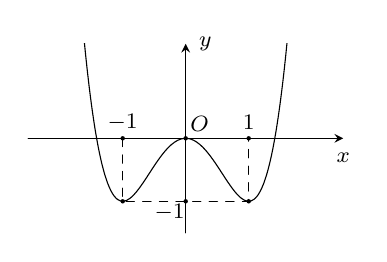
\begin{tikzpicture}[font=\footnotesize,line join=round, line cap=round, >=stealth,scale=0.8] 
\def \xmin{-2.5}\def \xmax{2.5}\def \ymin{-1.5}\def \ymax{1.5}
\draw[->] (\xmin,0)--(\xmax,0) node[shift=(-90:0.25)] {$x$};
\draw[->] (0,\ymin)--(0,\ymax) node[shift=(0:0.25)] {$y$};
\fill (0,0) circle(1pt) node[shift=(45:0.25)]{$O$}
	(-1,0) circle(1pt) node[shift=(90:0.2)]{$-1$}
	(1,0) circle(1pt) node[shift=(90:0.2)]{$1$}
	(0,-1) circle(1pt) node[shift=(-145:0.25)]{$-1$}
	(-1,-1) circle(1pt) (1,-1) circle(1pt);
\begin{scope}
\clip (\xmin,\ymin) rectangle (\xmax,\ymax);
\draw[smooth,samples=100,domain=\xmin:\xmax] plot(\x,{(\x)^4-2*(\x)^2}); 
\end{scope} 
\draw[dashed] (-1,0)--(-1,-1)--(1,-1)--(1,0);
\end{tikzpicture}}
\loigiai{
\immini{Ta có $\dfrac{3-f(x)}{1+f(x)}=5 \Leftrightarrow \dfrac{-2-6f(x)}{1+f(x)}=0 \Leftrightarrow f(x)=-\dfrac{1}{3}$.\\
Số nghiệm của phương trình $f(x)=-\dfrac{1}{3}$ là số giao điểm của đồ thị hàm số $y=f(x)$ và đường thẳng $y=-\dfrac{1}{3}$ vuông góc với trục tung tại điểm có tung độ bằng $-\dfrac{1}{3}$.\\
Từ đồ thị của hàm số $y=f(x)$, suy ra phương trình đã cho có đúng $4$ nghiệm thực phân biệt.}
{
\begin{tikzpicture}[font=\footnotesize,line join=round, line cap=round, >=stealth,scale=0.8] 
\def \xmin{-2.5}\def \xmax{2.5}\def \ymin{-1.5}\def \ymax{1.5}
\draw[->] (\xmin,0)--(\xmax,0) node[shift=(90:0.25)] {$x$};
\draw[->] (0,\ymin)--(0,\ymax) node[shift=(0:0.25)] {$y$};
\fill (0,0) circle(1pt) node[shift=(45:0.25)]{$O$}
	(-1,0) circle(1pt) node[shift=(90:0.2)]{$-1$}
	(1,0) circle(1pt) node[shift=(90:0.2)]{$1$}
	(0,-1) circle(1pt) node[shift=(-145:0.25)]{$-1$};
\begin{scope}
\clip (\xmin,\ymin) rectangle (\xmax,\ymax);
\draw[smooth,samples=100,domain=\xmin:\xmax] plot(\x,{(\x)^4-2*(\x)^2}); 
\end{scope} 
\draw[dashed] (-1,0)--(-1,-1)--(1,-1)--(1,0);
\draw (\xmin,-1/3)--(\xmax,-1/3)node[shift=(-90:0.25)] {$y=-\tfrac{1}{3}$};
\end{tikzpicture}}
}
\end{ex}

\begin{ex}%[Đề thi thử Tốt Nghiệp, Liên trường Lê Thánh Tông - Nguyễn Khuyến, HCM, 2023]%[12-EX-6-2023, Trần Quốc]%[2H1B3-3]
Cho tứ diện $ABCD$ có thể tích là $8a^3$. Gọi $M$, $N$ lần lượt là trung điểm của các cạnh $AB$ và $AC$. Thể tích khối đa diện $BCDMN$ bằng
\choice
{$3a^3$}
{$4a^3$}
{$5a^3$}
{\True $6a^3$}
\loigiai{
\immini{Ta có
$$ \dfrac{V_{A.MND}}{V_{A.BCD}}=\dfrac{AM}{AB}\cdot \dfrac{AN}{AC}=\dfrac{1}{4} \Rightarrow V_{A.MND}=\dfrac{1}{4}V_{A.BCD}=2a^3.$$
Suy ra $V_{BCDMN}=V_{A.BCD}-V_{A.MND}=6a^3$.
}
{
\begin{tikzpicture}[font=\footnotesize,line join=round, line cap=round, >=stealth,scale=0.8]
\tkzDefPoints{2/3/A, 0/0/B, 1.5/-1.5/C, 4/0/D}
\path ($(A)!1/2!(B)$) coordinate (M) ($(A)!1/2!(C)$) coordinate (N); 
\draw[dashed] (B)--(D)--(M); 
\draw (C)--(A)--(B)--(C)--(D)--(A) (M)--(N)--(D);
\foreach \x/\pos in {A/90, B/-150, C/-90, D/-30, M/150, N/-150} \fill (\x) circle(1pt) node[{shift=(\pos:0.25)}]{$\x$}; 
\end{tikzpicture}}}
\end{ex}

\begin{ex}%[Đề thi thử Tốt Nghiệp, Liên trường Lê Thánh Tông - Nguyễn Khuyến, HCM, 2023]%[12-EX-6-2023, Trần Quốc]%[2D2B4-3]
Đồ thị của hàm số $y=2023^{x^2}$ {\bf không} cắt đường thẳng $y=m$ khi và chỉ khi
\choice
{$m \leq 2023$}
{$m<2023$}
{$m \leq 1$}
{\True $m<1$}
\loigiai
{Xét hàm số $f(x)=2023^{x^2}$ trên $\mathbb{R}$.\\
Ta có $f'(x)=2x\cdot 2023^{x^2}\ln 2023$.\\
Phươn trình $f'(x)=0 \Leftrightarrow x=0$.\\
Bảng biến thiên của hàm số $y=f(x)$
\begin{center}

\begin{tikzpicture}
\tkzTabInit[nocadre=false,lgt=1.3,espcl=2.2,deltacl=0.6]
{$x$ /.6,$f'(x)$ /.6,$f(x)$/2}
{$-\infty$, $0$, $+\infty$}
\tkzTabLine{,-,$0$,+,}
\tkzTabVar{+/$+\infty$, -/$1$, +/$+\infty$}
\end{tikzpicture}
\end{center}
Từ bảng biến thiên, suy ra đồ thị của hàm số $y=2023^{x^2}$ không cắt đường thẳng $y=m$ khi và chỉ khi $m<1$.}
\end{ex}

\begin{ex}%[Đề thi thử Tốt Nghiệp, Liên trường Lê Thánh Tông - Nguyễn Khuyến, HCM, 2023]%[12-EX-6-2023, Trần Quốc]%[2H3B1-3]
Trong KG $Oxyz$, phương trình mặt cầu $(S)$ có tâm $I(1; 9;-3)$ tiếp xúc với trục $Ox$ là
\choice
{$(x-1)^2+(y-9)^2+(z+3)^2=10$}
{$(x-1)^2+(y-9)^2+(z+3)^2=45$}
{$(x-1)^2+(y-9)^2+(z+3)^2=82$}
{\True $(x-1)^2+(y-9)^2+(z+3)^2=90$}
\loigiai{Gọi $M$ là điểm tiếp xúc của mặt cầu $(S)$ với trục $Ox$.\\
Khi đó, $M$ là hình chiếu vuông góc của $I$ lên $Ox$ nên $M(1; 0; 0)$ và bán kính mặt cầu là $R=IM=\sqrt{90}$.\\
Suy ra phương trình mặt cầu là $(x-1)^2+(y-9)^2+(z+3)^2=90$.}
\end{ex}

\begin{ex}%[Đề thi thử Tốt Nghiệp, Liên trường Lê Thánh Tông - Nguyễn Khuyến, HCM, 2023]%[12-EX-6-2023, Trần Quốc]%[2D2B6-4]
Ông A bị nhiễm một loại vi-rút nên phải nhập viện và được điều trị ngay lập tức. Kể từ ngày nhập viện, sau mỗi ngày điều trị thì lượng vi-rút trong cơ thể ông A giảm đi $10\%$ so với ngày trước đó. Hỏi sau ít nhất bao nhiêu ngày thì ông A sẽ được xuất viện, biết rằng ông A được xuất viện khi lượng vi-rút trong cơ thể không quá $30\%$ so với ngày nhập viện?
\choice
{$11$ ngày}
{\True $12$ ngày}
{$13$ ngày}
{$14$ ngày}
\loigiai{Theo giả thiết, sau mỗi ngày điều trị thì lượng vi-rút trong cơ thể ông A còn lại $r=90\%=0{,}9$ so với ngày trước đó.\\
Gọi $K$ và $K_n$ lần lượt là lượng vi-rút trong cơ thể ông A khi bắt đầu nhập viện và sau $n$ ngày điều trị.\\
Áp đụng công thức lãi suất kép, ta có $K_n=Kr^n=K\cdot 0{,}9^n $.\\
Theo yêu cầu bài toán, ta cần có $K_n \le 0{,}3K \Leftrightarrow 0{,}9^n \le 0{,}3 \Leftrightarrow n \ge \log_{0{,}9}0{,}3$.\\
Suy ra $n \ge 12$. Vậy sau ít nhất $12$ ngày thì ông A sẽ được xuất viện.
}
\end{ex}

\begin{ex}%[Đề thi thử Tốt Nghiệp, Liên trường Lê Thánh Tông - Nguyễn Khuyến, HCM, 2023]%[12-EX-6-2023, Trần Quốc]%[2D1B2-5]
Hàm số $f(x)=mx^4-(m+2) x^2+2023$ có đúng ba điểm cực trị khi và chỉ khi
\choice
{\True $\hoac{&m<-2 \\&m>0}$}
{$m>-2$}
{$m<0$}
{$-2<m<0$}
\loigiai{ Ta có $f'=(x)=4mx^3-2(m+2)x=2x\left(2mx^2-m-2\right)$.\\
Phương trình $f'(x)=0 \Leftrightarrow \hoac{&x = 0 \\ &2mx^2 - m - 2 = 0} \Leftrightarrow \hoac{&x=0 \\ &2mx^2=m+2.}$\\
Do đó, hàm số $f$ có đúng ba điểm cực trị khi và chi khi $\heva{&m \neq 0 \\ &\dfrac{m+2}{2m}>0} \Leftrightarrow \hoac{&m<-2 \\ &m>0.}$}
\end{ex}

\begin{ex}%[Đề thi thử Tốt Nghiệp, Liên trường Lê Thánh Tông - Nguyễn Khuyến, HCM, 2023]%[12-EX-6-2023, Trần Quốc]%[2D1K3-1]
\immini{Cho hàm số $y=g(x)$ có đồ thị như hình bên. Gọi $M$, $m$ lần lượt là giá trị lớn nhất và nhỏ nhất của hàm số $y=g\left(\sqrt{1+8 \sin^2 x}-2\right)$. Khi đó
\choice
{$M-m=2$}
{$M-m=1$}
{$M-m=6$}
{\True $M-m=4$}}
{
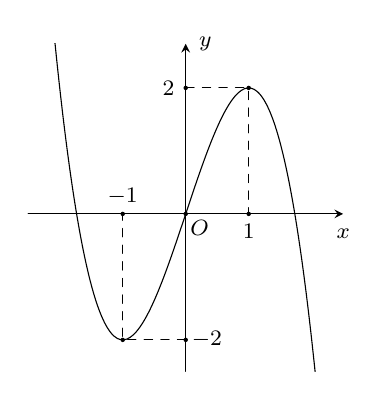
\begin{tikzpicture}[font=\footnotesize,line join=round, line cap=round, >=stealth,scale=0.8] 
\def \xmin{-2.5}\def \xmax{2.5}\def \ymin{-2.5}\def \ymax{2.7} 
\draw[->] (\xmin,0)--(\xmax,0) node[shift=(-90:0.25)] {$x$};
\draw[->] (0,\ymin)--(0,\ymax) node[shift=(0:0.25)] {$y$};
\fill (0,0) circle(1pt) node[shift=(-45:0.25)]{$O$}
		(-1,0) circle(1pt) node[shift=(90:0.22)]{$-1$}
		(1,0) circle(1pt) node[shift=(-90:0.22)]{$1$}
		(0,-2) circle(1pt) node[shift=(0:0.27)]{$-2$}
		(0,2) circle(1pt) node[shift=(180:0.22)]{$2$}
		(-1,-2) circle(1pt) (1,2) circle(1pt); 
\begin{scope}
\clip (\xmin,\ymin) rectangle (\xmax,\ymax);
\draw[smooth,samples=100,domain=\xmin:\xmax] plot(\x,{-(\x)^3+3*(\x)}); 
\end{scope}
\draw[dashed] (0,-2)-|(-1,0) (0,2)-|(1,0);
\end{tikzpicture}}
\loigiai{Đặt $t=\sqrt{1+8 \sin ^2 x}-2$.\\
Với mọi $x \in \mathbb{R}$, ta có 
$$0 \leq \sin^2 x \le 1 \Rightarrow 1 \le 1+8 \sin^2 x \le 9 \Rightarrow 1 \le \sqrt{1+8 \sin^2 x} \le 3 \Rightarrow -1 \le \sqrt{1+8 \sin^2 x}-2 \le 1.$$
Do đó $t\in[-1; 1]$.\\
Hàm số đã cho trở thành $y=g(t)$, với $t \in[-1; 1]$.\\
Từ đồ thị hàm số $y=g(x)$, ta suy ra giá trị lớn nhất là $M=2$ khi $t=1$ và giá trị nhỏ nhất là $m=-2$ khi $t=-1$.\\
Vậy $M-m=4$.}
\end{ex}

\begin{ex}%[Đề thi thử Tốt Nghiệp, Liên trường Lê Thánh Tông - Nguyễn Khuyến, HCM, 2023]%[12-EX-6-2023, Trần Quốc]%[2H2K2-1]
Cho hình chóp $S.ABCD$ có đáy $ABCD$ là hình vuông cạnh bằng $a$, tam giác $SAB$ đều và tam giác $SCD$ vuông tại $S$. Diện tích mặt cầu có tâm $S$ và tiếp xúc với mặt phẳng $(ABCD)$ bằng
\choice
{\True $\dfrac{3a^2}{4} \pi$}
{$\dfrac{4a^2}{3} \pi$}
{$\dfrac{3a^2}{2} \pi$}
{$3a^2 \pi$}
\loigiai{
\immini{
Gọi $M$, $N$ lần lượt là trung điểm của $AB$, $CD$ và $H$ là chân đường cao của $\triangle SMN$.\\
Vì $\triangle SAB$ là tam giác đều nên $SM \perp AB$.\\
Ta lại có $AB \perp MN$. Do đó $AB \perp (SMN) \Rightarrow (SMN) \perp (ABCD)$.\\
Mặt khác $\heva{&(SMN) \cap (ABCD)=MN \\ &SH \subset (SMN), SH \perp MN} \Rightarrow SH \perp (ABCD)$.\\
Suy ra mặt cầu có tâm $S$ và tiếp xúc với mặt phẳng $(ABCD)$ có bán kính $R=IH$.\\
Vì $\triangle SAB$ là tam giác đều cạnh $a$ nên $SM=\dfrac{AB\sqrt{3}}{2}=\dfrac{a\sqrt{3}}{2}$.\\
Vì $ABCD$ là hình vuông cạnh bằng $a$ nên $MN=a$.\\
Xét $\triangle SCD$ có $SN$ vừa là trung tuyến, vừa là đường cao nên $\triangle SCD$ vuông cân tại $S$, do đó $SN=\dfrac{1}{2}CD=\dfrac{a}{2}$.\\
Xét $\triangle SMN$ có $SM^2+SN^2=MN^2=a^2$, suy ra $\triangle SMN$ vuông tại $S$. \\
Do đó
$$ \dfrac{1}{SH^2}=\dfrac{1}{SM^2}+\dfrac{1}{SN^2}=\dfrac{4}{3a^2}+\dfrac{4}{a^2}=\dfrac{16}{3a^2} \Rightarrow R=SH=\dfrac{a\sqrt{3}}{4}. $$
Vậy diện tích mặt cầu cần tìm 
$$ S=4\pi R^2 =4\pi \dfrac{3a^2}{16}=\dfrac{3a^2}{4}\pi.$$
}
{
\begin{tikzpicture}[font=\footnotesize,line join=round, line cap=round, >=stealth,scale=0.8] 
\foreach \x/\y/\pos in {0/0/B, 1.5/2/A, 3.5/0/C} \path ($(\x,\y)$) coordinate (\pos); 
\path ($(A)+(C)$) coordinate (D)
		($(A)!1/2!(B)$) coordinate (M)
		($(C)!1/2!(D)$) coordinate (N)
		($(A)!1/2!(C)$) coordinate (H)
		($(H)+(0,4)$) coordinate (S);
\draw[dashed] (B)--(A)--(D) (A)--(S)--(M)--(N) (S)--(H);
\draw (C)--(S)--(B)--(C)--(D)--(S)--(N);
\foreach \x/\pos in {S/90, A/-90, B/-150, C/-30, D/0, M/-60, N/-30, H/-90} \fill (\x) circle(1pt) node[{shift=(\pos:0.25)}]{$\x$}; 
\end{tikzpicture}}
}
\end{ex}

\begin{ex}%[Đề thi thử Tốt Nghiệp, Liên trường Lê Thánh Tông - Nguyễn Khuyến, HCM, 2023]%[12-EX-6-2023, Trần Quốc]%[2D3K3-1]
Cho hàm số $y=f(x)$ có đạo hàm liên tục trên đoạn $[0;8]$ và có đồ thị như hình vẽ
\begin{center}
\begin{tikzpicture}[font=\footnotesize,line join=round, line cap=round, >=stealth,scale=0.8] 
\def \xmin{-1}\def \xmax{9}\def \ymin{-1}\def \ymax{4}
\draw[->] (\xmin,0)--(\xmax,0) node[shift=(-90:0.25)] {$x$};
\draw[->] (0,\ymin)--(0,\ymax) node[shift=(0:0.25)] {$y$};
\fill (0,0) circle(1pt) node[shift=(-135:0.25)]{$O$}
		(3,0) circle(1pt) node[shift=(-135:0.25)]{$3$}
		(5,0) circle(1pt) node[shift=(-45:0.25)]{$5$}
		(8,0) circle(1pt) node[shift=(-135:0.25)]{$8$}
		(0,3) circle(1pt) node[shift=(180:0.2)]{$3$}; 
\begin{scope}
\clip (\xmin,\ymin) rectangle (\xmax,\ymax); 
\draw[smooth,samples=100,domain=0:\xmax] plot(\x,{(\x+1)*(\x-3)*(\x-5)*(8-\x)/40}); 
\fill[pattern = north east lines,opacity=.5] plot[domain=0:3](\x,{(\x+1)*(\x-3)*(\x-5)*(8-\x)/40})--(0,0);
\fill[pattern = north west lines,opacity=.5] plot[domain=3:5](\x,{(\x+1)*(\x-3)*(\x-5)*(8-\x)/40})--(3,0);
\fill[pattern = north east lines,opacity=.5] plot[domain=3:5](\x,{(\x+1)*(\x-3)*(\x-5)*(8-\x)/40})--(3,0);
\fill[pattern = north west lines,opacity=.5] plot[domain=5:8](\x,{(\x+1)*(\x-3)*(\x-5)*(8-\x)/40})--(5,0);
\end{scope}
\draw[->] (2.5,2)node[right]{$S_1$}--(1.5,1.5);
\draw[->] (4,1)node[above]{$S_2$}--(4,-0.2);
\draw[->] (5.5,1)node[left]{$S_3$}--(6.5,1); 
\end{tikzpicture}
\end{center}
Biết $S_1=23$, $S_2=3$, $S_3=15$ lần lượt là diện tích hình phẳng giới hạn bởi đồ thị $y=f(x)$ và trục $Ox$. Giá trị của $I=\int\limits_5^6\left(-2x^3+9x^2-9x\right) f'\left(x^2-3x-10\right) \mathrm{\, d} x$ là
\choice
{$I=-15$}
{\True $I=65$}
{$I=5$}
{$I=35$}
\loigiai{Theo giả thiết, ta có 
\begin{itemize}
\item $\int\limits_{0}^{3}f(x)\mathrm{\, d} x=S_1=23$;
\item $\int\limits_{3}^{5}f(x)\mathrm{\, d} x=-S_2=-3$;
\item $\int\limits_{5}^{8}f(x)\mathrm{\, d} x=S_3=15$.
\end{itemize}
Suy ra $\int\limits_{0}^{8}f(x)\mathrm{\, d} x=\int\limits_{0}^{3}f(x)\mathrm{\, d} x+\int\limits_{3}^{5}f(x)\mathrm{\, d} x+\int\limits_{5}^{8}f(x)\mathrm{\, d} x=23-3+15=35$.\\
Xét $I=\int\limits_{5}^{6}\left(-2x^3+9x^2-9x\right) f'\left(x^2-3x-10\right) \mathrm{\, d} x=\int\limits_{5}^{6}\left(-x^2+3x\right)(2x-3)f'\left(x^2-3x-10\right) \mathrm{\, d} x$.\\
Đặt $t=x^2-3x-10 \Rightarrow \mathrm{d} t=(2x-3)\mathrm{\, d} x$.\\
Đổi cận $x=5 \Rightarrow t=0$; $x=6 \Rightarrow t=8$.\\
Khi đó, ta có $I=\int\limits_{0}^{8}(-t-10)f'(t)\mathrm{\, d} t$.\\
Đặt $\heva{&u=-t-10 \\&\mathrm{d} v=f'(t)\mathrm{\, d} t} \Rightarrow \heva{&\mathrm{d} u=-\mathrm{d} t \\& v=f(t)}$. Khi đó
$$ I=(-t-10)f(t)\Bigg|_{0}^{8}+\int\limits_{0}^{8}f(t)\mathrm{\, d} t=\left[-18f(8)+10f(0)\right]+35=(0+10\cdot 3)+35=65. $$
}
\end{ex}

\begin{ex}%[Đề thi thử Tốt Nghiệp, Liên trường Lê Thánh Tông - Nguyễn Khuyến, HCM, 2023]%[12-EX-6-2023, Trần Quốc]%[2D1K2-2]
\immini{Cho hàm số $y=f(x)=ax^3+bx+c$ có đồ thị như hình vẽ bên. Số điểm cực trị của hàm số $y=f\left(|x|\right)+2023$ là
\choice
{$2$}
{\True $3$}
{$7$}
{$5$}}
{
\begin{tikzpicture}[font=\footnotesize,line join=round, line cap=round, >=stealth,scale=0.8] 
\def \xmin{-3.5}\def \xmax{2.5}\def \ymin{-3}\def \ymax{1.5} 
\draw[->] (\xmin,0)--(\xmax,0) node[shift=(-90:0.25)] {$x$};
\draw[->] (0,\ymin)--(0,\ymax) node[shift=(0:0.25)] {$y$};
\fill (0,0) circle(1pt) node[shift=(-135:0.25)]{$O$};
\begin{scope}
\clip (\xmin,\ymin) rectangle (\xmax,\ymax);
\draw[smooth,samples=100,domain=\xmin:\xmax] plot(\x,{(\x+2)*(0.5-\x)*(\x-1.5)/1.5}); 
\end{scope}
\end{tikzpicture}}
\loigiai{
\immini{Số điểm cực trị của hàm số $y=f\left(|x|\right)+2023$ cũng là số điểm cực trị của hàm số $y=f\left(|x|\right)$.\\
Ta có $y=f\left(|x|\right)=\heva{&f(x) &\text{ nếu } x\ge 0 \\&f(-x) &\text{ nếu }x<0.}$\\
Do đó, đồ thị hàm số $y=f\left(|x|\right)$ gồm hai phần 
\begin{enumerate}[\bf Phần 1:]
\item Trùng phần đồ thị của hàm số $y=f(x)$ bên phải trục $Oy$;
\item Đối xứng với phần $1$ qua trục $Oy$.
\end{enumerate}
Từ đồ thị hàm số $y=f\left(|x|\right)$, suy ra hàm số $y=f\left(|x|\right)+2023$ có đúng $3$ điểm cực trị.}
{
\begin{tikzpicture}[font=\footnotesize,line join=round, line cap=round, >=stealth,scale=0.8] 
\def \xmin{-3.5}\def \xmax{2.5}\def \ymin{-3}\def \ymax{1.5} 
\draw[->] (\xmin,0)--(\xmax,0) node[shift=(-90:0.25)] {$x$};
\draw[->] (0,\ymin)--(0,\ymax) node[shift=(0:0.25)] {$y$};
\fill (0,0) circle(1pt) node[shift=(135:0.25)]{$O$}
		(0,-1) circle(1pt);
\begin{scope}
\clip (\xmin,\ymin) rectangle (\xmax,\ymax);
\draw[smooth,samples=200,domain=\xmin:\xmax] plot(\x,{(abs(\x)+2)*(0.5-abs(\x))*(abs(\x)-1.5)/1.5}); 
\end{scope}
\end{tikzpicture}}
}
\end{ex}

\begin{ex}%[Đề thi thử Tốt Nghiệp, Liên trường Lê Thánh Tông - Nguyễn Khuyến, HCM, 2023]%[12-EX-6-2023, Trần Quốc]%[2H2K1-2]
Một hình trụ được cắt bởi một mặt phẳng song song với trục và cách trục một khoảng bằng $\sqrt{5}$, thiết diện thu được là hình vuông có diện tích bằng $16$ . Tính thể tích $V$ của khối trụ đó.
\choice
{$V=28 \pi$}
{$V=32 \pi$}
{\True $V=36 \pi$}
{$V=44 \pi$}
\loigiai{\immini{Gọi $O$, $O'$ lần lượt là tâm hai đáy, $ABB'A'$ thiết diện hình vuông có cạnh bằng $a$ và $M$ là trung điểm $AB$ (như hình vẽ).\\
Theo giả thiết, ta có $a^2=16 \Rightarrow a=4$. Do đó $h=OO'=AA'=a=4$.\\
Khoảng cách từ trục của hình trụ đến thiết diện là $OM=\sqrt{5}$, suy ra
$$
r=OA=\sqrt{OM^2+AM^2}=\sqrt{(\sqrt{5})^2+\left(\frac{a}{2}\right)^2}=\sqrt{9}=3.
$$
Vậy thể tích khối trụ là $V=\pi r^2 h=9 \pi \cdot 4=36 \pi$.}
{
\begin{tikzpicture}[scale=0.6, font=\footnotesize,line join=round, line cap=round, >=stealth]
					\def\major{3} 
					\def\minor{0.8} 
					\def\height{4} 
					\path (0,0) coordinate(O') (90:\height) coordinate (O)
							($(O) + (105:{\major} and {\minor})$) coordinate (A)
							($(O') + (105:{\major} and {\minor})$) coordinate (A')
							($(O) + (-135:{\major} and {\minor})$) coordinate (B)
							($(O') + (-135:{\major} and {\minor})$) coordinate (B')
							($(A)!1/2!(B)$) coordinate (M);
					\draw[dashed] (\major,0) arc(0:180:{\major} and {\minor});
					\draw[dashed] (B')--(A')--(A) (O')--(O);
					\draw (\major,\height)--(\major,0) arc(0:-180:{\major} and {\minor})--(-\major,\height) arc(180:-180:{\major} and {\minor}) (A)--(B)--(B') (O)--(M);
				\foreach \x/\pos in {O/0, O'/0, A/90, B/-150, A'/150, B'/-135, M/180} \fill (\x) circle(1pt) node[{shift=(\pos:0.25)}]{$\x$}; 
			\draw pic[draw,angle radius=2mm] {right angle = B--M--O}; 
\end{tikzpicture}}}
\end{ex}

\begin{ex}%[Đề thi thử Tốt Nghiệp, Liên trường Lê Thánh Tông - Nguyễn Khuyến, HCM, 2023]%[12-EX-6-2023, Trần Quốc]%[1D2K5-2]
Một hộp gồm $23$ quả cầu được đánh số từ $1$ đến $23$. Lấy ngẫu nhiên $2$ quả cầu từ hộp đó. Xác suất để lấy được $2$ quả cầu và tích hai số ghi trên $2$ quả cầu đó là một số chia hết cho $6$ bằng
\choice
{$\dfrac{8}{23}$}
{\True $\dfrac{95}{253}$}
{$\dfrac{4}{11}$}
{$\dfrac{98}{253}$}
\loigiai{Lấy ngẫu nhiên $2$ quả cầu từ $23$ quả cầu, ta có số phần tử không gian mẫu là $\mathrm{C}_{23}^{2}$.\\
Gọi $A$ là biến cố \lq\lq  lấy được $2$ quả cầu và tích hai số ghi trên $2$ quả cầu đó là một số chia hết cho $6$\rq\rq .\\
Ta chia các quả cầu thành $3$ nhóm:
\begin{description}
\item[Nhóm 1:] Gồm các quả cầu có số chia hết cho $6$. \\
Nhóm này có $3$ quả cầu được đánh số là $6$, $12$, $18$;
\item[Nhóm 2:] Gồm các quả cầu có số chia hết cho $3$ nhưng không chia hết cho $6$. \\
Nhóm này có $4$ quả cầu được đánh số là $3$, $9$, $15$, $21$;
\item [Nhóm 3:] Gồm các quả cầu có số chia hết cho $2$ nhưng không chia hết cho $6$. \\
Nhóm này có $8$ quả cầu được đánh số là $2$, $4$, $8$, $10$, $14$, $16$, $20$, $22$;
\item [Nhóm 4:] Gồm các quả cầu còn lại.
\end{description}
Các trường hợp thuận lợi của biến cố $A$ là:
\begin{enumerate}[\bf TH1:]
\item Cả $2$ quả cầu lấy được cùng thuộc nhóm $1$.\\
Trường hợp này có $\mathrm{C}_{3}^{2}$ cách.
\item Trong $2$ quả cầu lấy được có $1$ quả thuộc nhóm $1$ và $1$ quả không thuộc nhóm $1$.\\
Trường hợp này có $3\cdot 20$ cách.
\item Trong $2$ quả cầu lấy được có $1$ quả thuộc nhóm $2$ và $1$ quả thuộc nhóm $3$.\\
Trường hợp này có $4\cdot 8$ cách.
\end{enumerate}
Suy ra $n(A)=\mathrm{C}_{3}^{2}+3\cdot 20+4\cdot 8=95$.\\
Vậy xác suất cần tìm là $\mathrm{P}(A)=\dfrac{95}{\mathrm{C}_{23}^2}=\dfrac{95}{253}$.}
\end{ex}

\begin{ex}%[Đề thi thử Tốt Nghiệp, Liên trường Lê Thánh Tông - Nguyễn Khuyến, HCM, 2023]%[12-EX-6-2023, Trần Quốc]%[1H3K3-3]
Hình chóp $S.ABCD$ có đáy $ABCD$ là hình vuông, tam giác $SAB$ đều và $(SAB) \perp (ABCD)$. Đường thẳng $SD$ tạo với mặt phẳng $(ABCD)$ một góc $\alpha$ thì giá trị $\tan \alpha$ bằng
\choice
{\True $\dfrac{\sqrt{15}}{5}$}
{$\dfrac{\sqrt{5}}{5}$}
{$\dfrac{\sqrt{15}}{3}$}
{$\dfrac{2 \sqrt{3}}{5}$}
\loigiai{
\immini{Gọi cạnh hình vuông $ABCD$ là $a$ và $H$ là trung điểm của $AB$.\\
Vì $\triangle SAB$ đều nên có cạnh bằng $a$, $SH \perp AB$ và $SH=\dfrac{a\sqrt{3}}{2}$.\\
Xét $\triangle ADH$ vuông tại $A$, ta có
$$ DH=\sqrt{AH^2+AD^2}=\sqrt{\dfrac{a^2}{4}+a^2}=\dfrac{a\sqrt{5}}{2}.$$
Mặt khác, ta có $(SAB)\perp (ABCD)$ nên $SH \perp(ABCD)$, suy ra góc giữa $SD$ và $(ABCD)$ là $\widehat{SDH}$. \\
Xét $\triangle SDH$ vuông tại $H$, ta có 
$$\tan \alpha=\tan \widehat{SDH}=\dfrac{SH}{DH}=\dfrac{a\sqrt{3}}{2}\cdot  \dfrac{2}{a\sqrt{5}}=\dfrac{\sqrt{3}}{\sqrt{5}}=\dfrac{\sqrt{15}}{5}.$$}
{
\begin{tikzpicture}[font=\footnotesize,line join=round, line cap=round, >=stealth,scale=0.8] 
\tkzDefPoints{0/0/A, 2.5/2/B, 5/0/D} 
\path ($(B)+(D)$) coordinate (C)
		($(A)!1/2!(B)$) coordinate (H)
		($(H)+(0,4)$) coordinate (S);
\draw[dashed] (D)--(H)--(S)--(B) (A)--(B)--(C);
\draw (D)--(S)--(A)--(D)--(C)--(S);
\foreach \x/\pos in {S/90, A/-150, B/-90, C/-30, D/-30, H/-90} \fill (\x) circle(1pt) node[{shift=(\pos:0.25)}]{$\x$}; 
\draw pic[draw,angle radius=3mm] {right angle= D--H--S};
\draw pic[draw,angle radius=4mm] {angle= S--D--H};    
\node[shift=(140:0.6)] at (D){$\alpha$}; 
\end{tikzpicture}}
}
\end{ex}

\begin{ex}%[Đề thi thử Tốt Nghiệp, Liên trường Lê Thánh Tông - Nguyễn Khuyến, HCM, 2023]%[12-EX-6-2023, Trần Quốc]%[2D1K1-3]
Có tất cả bao nhiêu giá trị nguyên của tham số $m \in(-23; 0)$ sao cho hàm số $f(x)=\left(x^4-8\right) \mathrm{e}^x-mx^2-\left(m^2-9 m\right)x+2023$ luôn đồng biến trên khoảng $(2;5)$?
\choice
{$21$}
{$19$}
{\True $14$}
{$8$}
\loigiai{Ta có $f'(x)=4x^3\mathrm{e}^x+\left(x^4-8\right)\mathrm{e}^x-2mx-\left(m^2-9m\right)=\left(x^4+4x^3-8\right)\mathrm{e}^x-2mx-m^2+9m$.\\
Hàm số đã cho đồng biến trên $(2;5)$ khi và chỉ khi $f'(x) \ge 0$, $\forall x \in (2;5)$\\
Ta có $f''(x)=\left(4x^3+12x^2\right)\mathrm{e}^x+\left(x^4+4 x^3-8\right)\mathrm{e}^x-2m=\left(x^4+8x^3+12x^2-8\right)\mathrm{e}^x-2m$.\\
Vì $\heva{&x^4+8x^3+12x^2-8=x^4+12x^2+8\left(x^3-1\right)>0, \forall x \in(2; 5)\\ &-2m>0, \forall m \in(-23; 0)}$ nên $f''(x)>0$, $\forall x \in(2; 5)$.\\
Do đó, hàm số $f'(x)$ đồng biến trên $(2;5)$. Suy ra $\min\limits_{[2;5]}f'(x)=f'(2)=-m^2+5m+40\mathrm{e}^2$.\\
Yêu cầu bài toán tương đương 
$$\min\limits_{[2;5]}f'(x) \ge 0 \Leftrightarrow -m^2+5m+40\mathrm{e}^2 \ge 0 \Leftrightarrow \dfrac{5-\sqrt{25+160\mathrm{e}^2}}{2}\le m \le \dfrac{5+\sqrt{25+160\mathrm{e}^2}}{2}.$$
Do $m \in(-23; 0) \cap \mathbb{Z}$ nên $m \in\{-14;-15; \ldots . .;-2;-1\}$.\\
Vậy có tất cả $14$ giá trị nguyên của tham số $m \in(-23; 0)$ thỏa mãn bài toán.}
\end{ex}

\begin{ex}%[Đề thi thử Tốt Nghiệp, Liên trường Lê Thánh Tông - Nguyễn Khuyến, HCM, 2023]%[12-EX-6-2023, Trần Quốc]%[2D2K5-5]
\immini{Cho hàm số $y=f(x)$ liên tục trên $\mathbb{R}$ và có đồ thị như hình vẽ bên. Tổng tất cả các giá trị nguyên của tham số $m$ để phương trình $3f\left(2\log_{5}x\right)+6=m$ có đúng $3$ nghiệm thực thuộc nửa đoạn $\left(\dfrac{1}{25};25\right]$ bằng
\choice
{$69$}
{$57$}
{$60$}
{\True $66$}}
{
\begin{tikzpicture}[font=\footnotesize,line join=round, line cap=round, >=stealth,scale=0.6] 
\def \xmin{-5}\def \xmax{5}\def \ymin{-3.5}\def \ymax{4.7}
\draw[->] (\xmin,0)--(\xmax,0) node[shift=(-90:0.25)] {$x$};
\draw[->] (0,\ymin)--(0,\ymax) node[shift=(0:0.25)] {$y$};
\fill (0,0) circle(1pt) node[shift=(-135:0.25)]{$O$}
		(-4,0) circle(1pt) node[shift=(135:0.25)]{$-4$}
		(-3,0) circle(1pt) node[shift=(-90:0.18)]{$-3$}
		(-1.333,0) circle(1pt) node[shift=(-90:0.25)]{$-\tfrac{4}{3}$}
		(1,0) circle(1pt) node[shift=(-120:0.21)]{$1$}
		(2,0) circle(1pt) node[shift=(90:0.18)]{$2$}
		(4,0) circle(1pt) node[shift=(-90:0.18)]{$4$}
		(0,-3) circle(1pt) node[shift=(180:0.25)]{$-3$}
		(0,-1) circle(1pt) node[shift=(0:0.25)]{$-1$}
		(0,1) circle(1pt) node[shift=(180:0.2)]{$1$}
		(0,2) circle(1pt) node[shift=(0:0.17)]{$2$}
		(0,3) circle(1pt) node[shift=(45:0.2)]{$3$}
		(0,4) circle(1pt) node[shift=(0:0.17)]{$4$}
;
\begin{scope}
\clip (\xmin,\ymin) rectangle (\xmax,\ymax);
\foreach \x/\y/\pos in {-4/-1/A, -3/4/B, -1.333/2/C, 0/3/D, 2/-3/F, 4/1/G} \path ($(\x,\y)$) coordinate (\pos); 
\foreach \x in {A,B,C,F,G} \fill (\x) circle(1pt); 
\draw 
		(A) .. controls +(85:1) and +(180:.3) .. (B)
		.. controls +(0:.3) and +(180:0.3) .. (C)
		.. controls +(0:.25) and +(180:.25) .. (D)
		.. controls +(0:.5) and +(180:.5).. (F)
		..controls +(0:.5) and +(-95:.2) .. (G);
\end{scope} 
\draw[dashed] (-4,0)|-(0,-1) (-3,0)|-(0,4) (-1.333,0)|-(0,2) (2,0)|-(0,-3) (4,0)|-(0,1);
\end{tikzpicture}}
\loigiai{Đặt $t=2\log_{5}x$. Phương trình đã cho trở thành $ 3f(t)+6=m \Leftrightarrow f(t)=\dfrac{m-6}{3}$.\\
Với mọi $x \in \left(\dfrac{1}{25};25\right]$, ta có $t \in (-4;4]$ và tương ứng mỗi giá trị $t$, ta có một giá trị $x$.\\
Do đó, phương trình đã cho có đúng $3$ nghiệm thực thuộc $\left(\dfrac{1}{25};25\right]$ khi và chỉ khi phương trình $f(t)=\dfrac{m-6}{3}$ có đúng $3$ nghiệm thực thuộc $(-4;4]$.\\
Từ đồ thị hàm số $y=f(x)$, ta suy ra 
$$ \hoac{&-1 <\dfrac{m-6}{3}\le 1 \\&\dfrac{m-6}{3}=2 \\&\dfrac{m-6}{3}=3}\Leftrightarrow \hoac{&3<m \le 9 \\& m=12\\&m=15.} $$
Vì $m\in \mathbb{Z}$ nên ta có $m\in \{4;5;6;7;8;9;12;15\}$.\\
Vậy tổng các giá trị của tham số $m$ là $S=4+5+6+7+8+9+12+15=66$.
}
\end{ex}

\begin{ex}%[Đề thi thử Tốt Nghiệp, Liên trường Lê Thánh Tông - Nguyễn Khuyến, HCM, 2023]%[12-EX-6-2023, Trần Quốc]%[2H3K3-6]
Trong KG $Oxyz$, gọi $d'$ là hình chiếu vuông góc của $d\colon \heva{&x=-1+2at \\ &y=3-2t \\ &z=\left(a^2-2\right)t}$, $\left(t\in \mathbb{R}\right)$ lên mặt phẳng $(\alpha) \colon 2x-3z-6=0$. Lấy các điểm $M(0;-3;-2)$, $N(3;-1; 0)$ thuộc $(\alpha)$. Tính tổng tất cả các giá trị của tham số $a$ để $MN \perp d'$.
\choice
{\True $-4$}
{$-3$}
{$1$}
{$2$}
\loigiai{
Ta có $\overrightarrow{MN}=(3;2;2)$ và đường thẳng $d$ có một véc-tơ chỉ phương là $\overrightarrow{u}_{d}=\left(2a; -2; a^2-2\right)$.\\
Vì $d'$ là hình chiếu vuông góc của $d$ lên mặt phẳng $\alpha$ nên $MN \perp d'$ khi và chỉ khi $MN \perp d$.\\
Do đó, ta có $\overrightarrow{MN}\cdot \overrightarrow{u}_{d}=0 \Leftrightarrow 3\cdot 2a+2\cdot (-2)+2\cdot \left(a^2-2\right)=0 \Leftrightarrow 2a^2+6a-8=0 \Leftrightarrow \hoac{&a=1 \\&a=-4.}$\\
Vậy tích các giá trị của tham số $a$ là $P=1\cdot (-4)=-4$.
}
\end{ex}

\begin{ex}%[Đề thi thử Tốt Nghiệp, Liên trường Lê Thánh Tông - Nguyễn Khuyến, HCM, 2023]%[12-EX-6-2023, Trần Quốc]%[2D3G3-1]
Cho hàm số $f$ thỏa mãn $\heva{&f(x)>0 \\ &\mathrm{e}^{1-x^2}\left[6 f(x)+f'(x)\right]=\left(8x^2+12x+4\right) \sqrt{f(x)}}$, $\forall x>0$ và $f(1)=4$. Hình phẳng được giới hạn bởi $y=\sqrt{f(x)}$, $x=1$, $x=3$ và trục hoành có diện tích bằng $m \cdot \mathrm{e}^n+p$, trong đó $m$, $n$, $p \in \mathbb{Z}$. Hệ thức nào sau đây đúng?
\choice
{$2m+n+p=6$}
{\True $5m-n-3p=0$}
{$3m+n-p=15$}
{$3m+2n-p=19$}
\loigiai{Với mọi $x>0$, ta có
\begin{eqnarray*}
&&\mathrm{e}^{1-x^2}\left[6 f(x)+f'(x)\right]=\left(8x^2+12x+4\right) \sqrt{f(x)}\\
&\Leftrightarrow & \dfrac{6f(x)+f'(x)}{\sqrt{f(x)}}=\left(8x^2+12x+4\right)\mathrm{e}^{x^2-1}\\
&\Leftrightarrow & 3\sqrt{f(x)}+\dfrac{f'(x)}{2\sqrt{f(x)}}=\left(4x^2+6x+2\right)\mathrm{e}^{x^2-1} \\
& \Leftrightarrow & 3\mathrm{e}^{3x}\sqrt{f(x)}+\mathrm{e}^{3x} \dfrac{f'(x)}{2\sqrt{f(x)}}=\left(4x^2+6x+2\right)\mathrm{e}^{x^2+3x-1} \\
& \Leftrightarrow & 3\mathrm{e}^{3x} \sqrt{f(x)}+ \mathrm{e}^{3 x} \dfrac{f'(x)}{2\sqrt{f(x)}}=2\mathrm{e}^{x^2+3x-1}+2x\left(2x+3\right) \mathrm{e}^{x^2+3x-1} \\
& \Leftrightarrow & \left(\mathrm{e}^{3x} \sqrt{f(x)}\right)'=\left(2x \cdot \mathrm{e}^{x^2+3x-1}\right)' \\
& \Leftrightarrow & \mathrm{e}^{3x} \sqrt{f(x)}=2x \cdot \mathrm{e}^{x^2+3 x-1}+C.
\end{eqnarray*}
Với $x=1$, ta có $\mathrm{e}^3\sqrt{4}=2\mathrm{e}^3+C \Leftrightarrow C=0$.\\
Do đó $\sqrt{f(x)}=2x \cdot \mathrm{e}^{x^2-1}$, $\forall x>0$.\\
Diện tích hình phẳng được giới hạn bởi $y=\sqrt{f(x)}$, $x=1$, $x=3$ và trục hoành là
$$
S=\int\limits_1^3\left|2x\cdot\mathrm{e}^{x^2-1}\right| \mathrm{\, d} x=\int\limits_1^3 2x \cdot \mathrm{e}^{x^2-1} \mathrm{\, d} x=\int\limits_1^3 \mathrm{e}^{x^2-1} \mathrm{\, d}\left(x^2-1\right)=\mathrm{e}^{x^2-1}\Big|_1 ^3=\mathrm{e}^8-1.
$$
Suy ra $m=1$, $n=8$ và $p=-1$. Vậy $5m-n-3p=5-8-3(-1)=0$.}
\end{ex}

\begin{ex}%[Đề thi thử Tốt Nghiệp, Liên trường Lê Thánh Tông - Nguyễn Khuyến, HCM, 2023]%[12-EX-6-2023, Trần Quốc]%[2D1G2-2]
Cho hàm số $y=f(x)$ có đạo hàm trên $\mathbb{R}$ và có bảng biến thiên như sau
\begin{center}

\begin{tikzpicture}
\tkzTabInit[nocadre=false,lgt=1.2,espcl=2,deltacl=0.6] 
{$x$ /.6,$f(x)$/2}
{$-\infty$, $-15$, $-12$, $1$, $3$, $4$, $+\infty$}
\tkzTabVar{-/$-\infty$, +/$3$, -/$0$, +/$5$, -/$-5$, +/$3$, -/$-\infty$} 
\end{tikzpicture}
\end{center}
Số điểm cực đại của hàm số $g(x)=\left|f\left(\left|2x^2-6x-8\right|+x^2-13\right)\right|$ là
\choice
{\True $8$}
{$10$}
{$9$}
{$7$}
\loigiai{
Đặt $u(x)=\left|2x^2-6x-8\right|+x^2-13$.\\
Khi đó, ta có $u'(x)=\dfrac{(4x-6)\left(2x^2-6x-8\right)}{\left|2x^2-6x-8\right|}+2x$, $x\notin \{-1; 4\}$.\\
Phương trình $u'(x)=0 \Leftrightarrow x=3$.\\
Bảng biến thiên của hàm số $y=u(x)$
\begin{center}

\begin{tikzpicture}
\tkzTabInit[nocadre=false,lgt=1.3,espcl=2.2,deltacl=0.6] 
{$x$ /.6,$u'(x)$ /.6,$u(x)$/2}
{$-\infty$, $-1$, $3$, $4$, $+\infty$}
\tkzTabLine{,-,d,+,$0$,-,d,+,}
\tkzTabVar{+/$+\infty$, -/$-12$, +/$4$, -/$3$, +/$+\infty$} 
\end{tikzpicture}
\end{center}
Xét hàm số $h(x)=f\left(u(x)\right)$.\\
Ta có $h'(x)=u'(x)f'\left(u(x)\right)$, $x\notin \{-1; 4\}$.\\
Phương trình 
$$h'(x)=0 \Leftrightarrow \hoac{&u'(x)=0 \\&f'\left(u(x)\right)=0} 
\Leftrightarrow \hoac{&u'(x)=0 \\&u(x)=-15 &\text{ (vô nghiệm)}\\&u(x)=-12 \\&u(x)=1 \\&u(x)=3 \\&u(x)=4} 
\Leftrightarrow \hoac{&x=3 &\text{ (bội $3$)} \\ &x=-1 &\text{ (loại)}\\ &x=\dfrac{3-5\sqrt{3}}{3}& \\&x=3-\sqrt{3}& \\ &x=-2& \\&x=2 & \\ &x=4 &\text{ (loại)} \\&x=\dfrac{3-2\sqrt{21}}{3}& \\&x=\dfrac{3+2\sqrt{21}}{3}.&}$$
Phương trình 
$$ h(x)=0 \Leftrightarrow f\left(u(x)\right)=0 \Leftrightarrow \hoac{&u(x)=a\in (-\infty; -15) &\text{ (vô nghiệm)} \\&u(x)=-12 &\text{ (nghiệm bội chẵn)}\\&u(x)=b\in (1;3) &\text{ (hai nghiệm phân biệt)} \\&u(x)=c \in (3;4) &\text{ (bốn nghiệm phân biệt)} \\&u(x)=d \in (4;+\infty) &\text{ (hai nghiệm phân biệt).}} $$
Suy ra hàm số $g(x)=\left|h(x)\right|$ có tất cả $9+8=17$ điểm cực trị.\\
Mặt khác, vì $\lim\limits_{x \to +\infty} g(x)=+\infty$ nên hàm số có $8$ điểm cực đại và $9$ điểm cực tiểu. 
}
\end{ex}

\begin{ex}%[Đề thi thử Tốt Nghiệp, Liên trường Lê Thánh Tông - Nguyễn Khuyến, HCM, 2023]%[12-EX-6-2023, Trần Quốc]%[2D2G6-3]
Xét các số thực $x$, $y$ sao cho $27y^2+\log _{216}\left(a^{18x-\log_6 a^3}\right)^3 \le 783$ luôn đúng với mọi $a>0$. Có tối đa bao nhiêu giá trị nguyên dương $K=x^2+y^2-2x+5y$?
\choice
{$64$}
{$53$}
{\True $58$}
{$59$}
\loigiai{Ta có
\begin{eqnarray*}
&&27y^2+\log _{216}\left(a^{18x-\log_6 a^3}\right)^3 \le 783\\
&\Leftrightarrow &27y^2+3\log _{216}\left(a^{18x-\log_6 a^3}\right) \le 783\\
&\Leftrightarrow &9y^2+\left(18x-\log_6 a^3\right)\log _{6^3}a -261\le 0\\
&\Leftrightarrow &9y^2+\left(6x-\log_6 a\right)\log _{6}a -261\le 0\\
&\Leftrightarrow &-\log_6^2 a+6x\log_6 a+9y^2-261 \le 0. \qquad (1)
\end{eqnarray*}
Đặt $t=\log_6 a$, $(1)$ trở thành $-t^2+6xt+9y^2-261 \le 0$ . \qquad $(2)$\\
Bất phương trình $(1)$ đúng với mọi $a>0$ khi và chỉ khi bất phương trình $(2)$ đúng với mọi $t \in \mathbb{R}$. Khi đó, ta có
$$ \heva{&a<0 \\&\Delta'\le 0} \Leftrightarrow \heva{&-1<0 \text{ (luôn đúng)} \\&9x^2+9y^2-261\le 0} \Leftrightarrow x^2+y^2\le 29. \qquad (3)$$
Trên mặt phẳng tọa độ $Oxy$, tập hợp điểm $M(x;y)$ có tọa độ thỏa bất phương trình $(3)$ là hình tròn $\left(C_1\right)$ tâm $I_1(0;0)$ và bán kính $R_1=\sqrt{29}$.\\
Giả sử tồn tại số nguyên dương $K$ thỏa mãn $K=x^2+y^2-2x+5y$. Khi đó, ta có
$$ (x-1)^2+\left(y+\dfrac{5}{2}\right)^2=\dfrac{29}{4}+K. $$
Với $K$ là số nguyên dương, ta luôn có $\dfrac{29}{4}+K > 0$.\\
Khi đó, điểm $M(x;y)$ cũng thuộc đường tròn $(C_2)$ có tâm $I_2\left(1;-\dfrac{5}{2}\right)$ và bán kính $R_2=\sqrt{\dfrac{29}{4}+K}$.\\
Điểm $M(x;y)$ tồn tại khi và chỉ khi $2$ đường tròn $(C_1)$ và $(C_2)$ có điểm chung, tương đương
\begin{eqnarray*}
\left|R_1-R_2\right| \le I_1I_2 \le R_1+R_2 &\Leftrightarrow& \left|\sqrt{29}-\sqrt{\dfrac{29}{4}+K}\right| \le \sqrt{1^2+\left(\dfrac{5}{2}\right)^2} \le \sqrt{29}+\sqrt{\dfrac{29}{4}+K}\\
&\Leftrightarrow & \left|\sqrt{29}-\sqrt{\dfrac{29}{4}+K}\right| \le \dfrac{\sqrt{29}}{2}\\
&\Leftrightarrow &-\dfrac{\sqrt{29}}{2}\le \sqrt{29}-\sqrt{\dfrac{29}{4}+K} \le \dfrac{\sqrt{29}}{2}\\
&\Leftrightarrow &\dfrac{\sqrt{29}}{2} \le \sqrt{\dfrac{29}{4}+K} \le \dfrac{3\sqrt{29}}{2}\\
&\Leftrightarrow &\dfrac{29}{4} \le \dfrac{29}{4}+K\le \dfrac{9\cdot 29}{4}\\
&\Leftrightarrow &0 \le K \le 58.
\end{eqnarray*}
Vậy có tất cả $58$ giá trị nguyên dương của $K$ thỏa mãn bài toán là $K \in \{1;2;\ldots;58\}$.
}
\end{ex}

\begin{ex}%[Đề thi thử Tốt Nghiệp, Liên trường Lê Thánh Tông - Nguyễn Khuyến, HCM, 2023]%[12-EX-6-2023, Trần Quốc]%[1H3G5-4]
Cho lăng trụ đứng $ABCD.A'B'C'D'$ có chiều cao bằng $4a$ và $ABCD$ là hình bình hành. Gọi $M$, $N$ lần lượt là trung điểm của cạnh $AA'$, $CD$. Khi mặt phẳng $\left(A'NB\right)$ tạo với mặt đáy của lăng trụ một góc là $60^{\circ}$ thì khoảng cách giữa hai đường thẳng $DM$ và $A'N$ bằng
\choice
{\True $a$}
{$\dfrac{a \sqrt{3}}{2}$}
{$a\sqrt{2}$}
{$\dfrac{a \sqrt{6}}{2}$}
\loigiai{
\immini{Gọi $E$ là trung điểm cạnh $AB$.\\
Khi đó, ta có $(MDE) \parallel \left(A'NB\right)$.\\
Suy ra 
$$\mathrm{d}(DM,A'N)=\mathrm{d}\left((DME),(A'BN)\right)=\mathrm{d}\left(B,(DME)\right)=\mathrm{d}\left(A,(DME)\right).$$
Kẻ $AI \perp DE$ tại $I$ và $AK \perp MI$ tại $K$.\\
Ta có $\heva{&DE \perp AI \\&DE \perp AM}$ nên $DE \perp MI$.\\
Do đó 
$$\left(\left(A'NB\right), (ABCD)\right)=\left((DME), (ABCD)\right)=(MI,AI)=\widehat{AIM}=60^{\circ}.$$
Xét $\triangle AMI$ vuông tại $A$, ta có
$$\tan \widehat{AIM}=\dfrac{AM}{AI} \Rightarrow AI=\dfrac{AM}{\tan \widehat{AIM}}=\dfrac{2a}{\tan 60^{\circ}}=\dfrac{2a\sqrt{3}}{3}.$$
Suy ra $\dfrac{1}{AK^2}=\dfrac{1}{AM^2}+\dfrac{1}{AI^2}=\dfrac{1}{4a^2}+\dfrac{3}{4a^2}=\dfrac{1}{a^2}$.\\
Vậy $\mathrm{d}\left(A'N, DM\right)=\mathrm{d}\left(A,(DME)\right)=AK=a$.}
{
\begin{tikzpicture}[font=\footnotesize,line join=round, line cap=round, >=stealth,scale=0.8] 
\foreach \x/\y/\pos in {0/0/A, 4/0/B, 1.5/1.7/D} \path ($(\x,\y)$) coordinate (\pos) ($(\x,\y)+(0,4)$) coordinate (\pos'); 
\path ($(B)+(D)$) coordinate (C)
		($(B')+(D')-(A')$) coordinate (C')
		($(D)!1/2!(C)$) coordinate (N)
		($(A)!1/2!(B)$) coordinate (E)
		($(A)!1/2!(A')$) coordinate (M)
		($(E)!2/5!(D)$) coordinate (I)
		($(M)!1/2!(I)$) coordinate (K);
\draw[dashed] (A)--(D)--(C) (D)--(D') (A')--(N)--(B) (E)--(D)--(M)--(I)--(A)--(K);
\draw (A')--(B')--(C')--(D')--(A')--(A)--(B)--(C)--(C') (B)--(B') (A')--(B) (M)--(E);
\foreach \x/\pos in {A/-150, B/-30, C/-30, D/45, A'/150, B'/-30, C'/30, D'/150, M/180, N/60, E/-90, I/30, K/45} \fill (\x) circle(1pt) node[{shift=(\pos:0.25)}]{$\x$}; 
\end{tikzpicture}}}
\end{ex}

\begin{ex}%[Đề thi thử Tốt Nghiệp, Liên trường Lê Thánh Tông - Nguyễn Khuyến, HCM, 2023]%[12-EX-6-2023, Trần Quốc]%[2H3G2-8]
Trong KG $Oxyz$, cho khối đa diện $OAMEN$ có thể tích $296$ với các đỉnh $A\left(0; 0; 8\sqrt{2}\right)$, $M(5; 0; 0)$, $N(0; 7; 0)$, $E(a; b; 0)$, trong đó $a$, $b$ là các số thực dương. Khi $a$, $b$ thay đổi thì đường thẳng $AE$ tiếp xúc với mặt cầu $(S) \colon x^2+y^2+z^2=c^2$. Mặt cầu $(S)$ có bán kính nhỏ nhất bằng
\choice
{$\dfrac{24 \sqrt{666}}{333}$}
{$\dfrac{81 \sqrt{37}}{74}$}
{$\dfrac{27 \sqrt{222}}{37}$}
{\True $\dfrac{24 \sqrt{74}}{\sqrt{461}}$}
\loigiai{
\immini{Ta có bốn điểm $O$, $M$, $N$ và $E$ cùng thuộc mặt phẳng $(Oxy)$.\\
Ta có $S_{\triangle OMN}=\dfrac{1}{2}OM\cdot ON=\dfrac{35}{2}$ và 
$$ S_{OMEN}=\dfrac{3V_{A.OMEN}}{OA}=\dfrac{3\cdot 396}{8\sqrt{2}}=\dfrac{111}{\sqrt{2}}. $$
Vì $S_{OMEN}>S_{\triangle OMN}$ nên điểm $E$ nằm ngoài tam giác $OMN$.\\
Mặt khác, ta có 
\begin{align*}
S_{OMEN}&=S_{\triangle EON}+S_{\triangle EOM}\\
&=\dfrac{1}{2}\cdot \left|x_{E}\right|\cdot ON +\dfrac{1}{2}\cdot \left|y_{E}\right|\cdot OM\\
&=\dfrac{7a+5b}{2}.
\end{align*}
Do đó $7a+5b=111\sqrt{2}$ hay $E$ thuộc đoạn thẳng $BC$ với $B\left(\dfrac{111\sqrt{2}}{7};0;0\right)$ và $C\left(0;\dfrac{111\sqrt{2}}{5};0\right)$.
}
{
\begin{tikzpicture}[font=\footnotesize,line join=round, line cap=round, >=stealth,scale=1] 
\foreach \x/\y/\pos in {0/0/O, 0/3/A, -1.5/-2/C, 4/0/B} \path ($(\x,\y)$) coordinate (\pos); 
\path ($(O)!3/5!(B)$) coordinate (M)
		($(O)!3/5!(C)$) coordinate (N)
		($(O)!4/3!(A)$) coordinate (z)
		($(O)!4/3!(B)$) coordinate (x)
		($(O)!4/3!(C)$) coordinate (y)
		($(B)!1.2/4!(C)$) coordinate (E)
		($(B)!1.1/2!(C)$) coordinate (I)
		($(A)!2.1/5!(I)$) coordinate (H)
		($(A)!2.1/5!(E)$) coordinate (K);
\draw[dashed] (B)--(O)--(C) (O)--(A) (H)--(O)--(K) (I)--(O)--(E) (M)--(E)--(N)--(M);
\foreach \x/\y/\pos in {A/z/0,B/x/-90,C/y/0}\draw[->] (\x)--(\y)node[shift=(\pos:0.25)]{$\y$}; 
\draw (A)--(B)--(C)--(A) (I)--(A)--(E) (H)--(K);
\foreach \x/\pos in {O/180, A/180, B/60, C/180, M/90, N/120, E/-45, H/180, K/30} \fill (\x) circle(1pt) node[{shift=(\pos:0.25)}]{$\x$}; 
\foreach \x/\y/\z in {O/I/C, O/H/K, O/K/E} \draw pic[draw,angle radius=2mm] {right angle= \x--\y--\z};  
\end{tikzpicture}}
\noindent Gọi $H$, $K$ lần lượt là hình chiếu vuông góc của $O$ lên $(ABC)$ và đường thẳng $AE$.\\
Vì $OA$, $OB$ và $OC$ đôi một vuông góc nên 
$$ \dfrac{1}{OH^2}=\dfrac{1}{OA^2}+\dfrac{1}{OB^2}+\dfrac{1}{OC^2}=\dfrac{1}{8^2\cdot 2}+\dfrac{7^2}{111^2\cdot 2}+\dfrac{5^2}{111^2\cdot 2}= \dfrac{461}{42624} \Rightarrow AH=\dfrac{24\sqrt{74}}{\sqrt{461}}.$$
Vì mặt cầu $(S)$ có tâm $O(0;0;0)$ và tiếp xúc đường thẳng $AE$ nên có bán kính 
$$ R=|c|=\mathrm{d}(O,AE)=OK \ge OH=\dfrac{24\sqrt{74}}{\sqrt{461}}. $$
Suy ra bán kính nhỏ nhất của mặt cầu $(S)$ là $R_{\min}=\dfrac{24\sqrt{74}}{\sqrt{461}}$ khi $K\equiv H$, khi đó $E$ là hình chiếu vuông góc của $O$ lên $AB$.
}
\end{ex}


\Closesolutionfile{ans}
\begin{indapan}{10}
	{ans/ans-2-TT-24-LeThanhTong-NguyenKhuyen-HCM-23}
\end{indapan}
